\section{Quantum GIS 1.0}
\pagenumbering{arabic}
\setcounter{page}{1}

Quantum GIS (QGIS) is a user friendly Open Source Geographic Information
System (GIS), licensed under the GNU General Public License, that runs on
GNU/Linux, Unix, Mac OSX, and MS Windows. QGIS supports numerous vector, 
raster, and database formats and provides a wide variety of plugins to do 
things like display tracks from your GPS, edit and analyse vector geometries 
and attribute data, compose print layouts, and much more.

\subsection{History and Facts}

QGIS began life in February of 2002, with the first release in June of the
same year. The initial goal was to create a viewer for PostGIS data that ran
on Linux. From those humble beginnings, QGIS has become a true cross-platform
application that runs on all major versions of unix, Linux, as well as Mac
and Windows. It supports editing and map composition as well as integration
with GRASS to provide powerful GIS capability. 

QGIS 1.0, released in January 2009 provides a stable API from which you can
develop custom solutions in Python or C++. Even though 1.0 is fresh, there
are a number of exciting developments underway in both the core application
and plugins.

\subsection{QGIS Community}

\begin{figure}[h]
   \begin{center}
   \caption{QGIS Community Map}\label{fig:community-map}\smallskip
   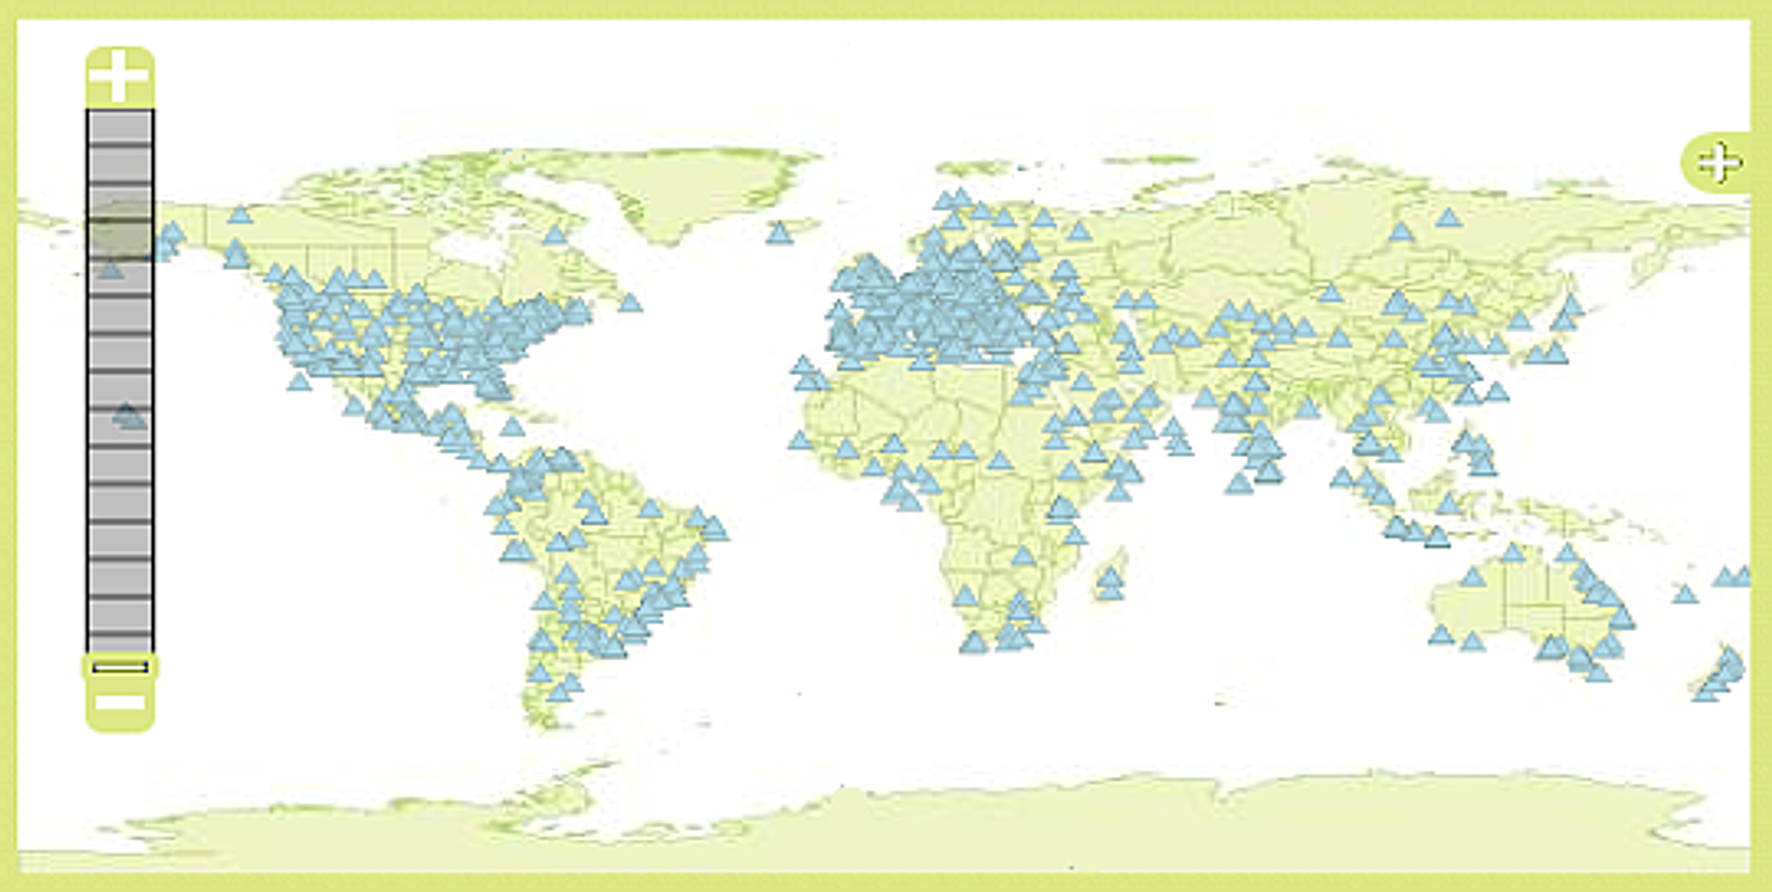
\includegraphics[clip=true]{community-map}
\end{center}
\end{figure}

\subsection{Functionality}



\subsection{Development}

\subsection{Conclusion}

\minisec{Authors}

The authors of this article are QGIS Project Steering Committee Members:

Otto Dassau <dassau@nature-consult.de>  
\\Gary Sherman <sherman@mrcc.com>
\\Tim Sutton <tim@linfinity.com>
\\Marco Hugentobler <marco.hugentobler@karto.baug.ethz.ch>
\\Paolo Cavallini <cavallini@faunalia.it>

\minisec{Links}

For more information, have a look at the following website:

Quantum GIS website: http://qgis.osgeo.org



 



